\chapter{Results}
\label{ch:testing}

\section{Simulation parameters}

\begin{figure} [h]
\centering
\hspace*{-1.0in}
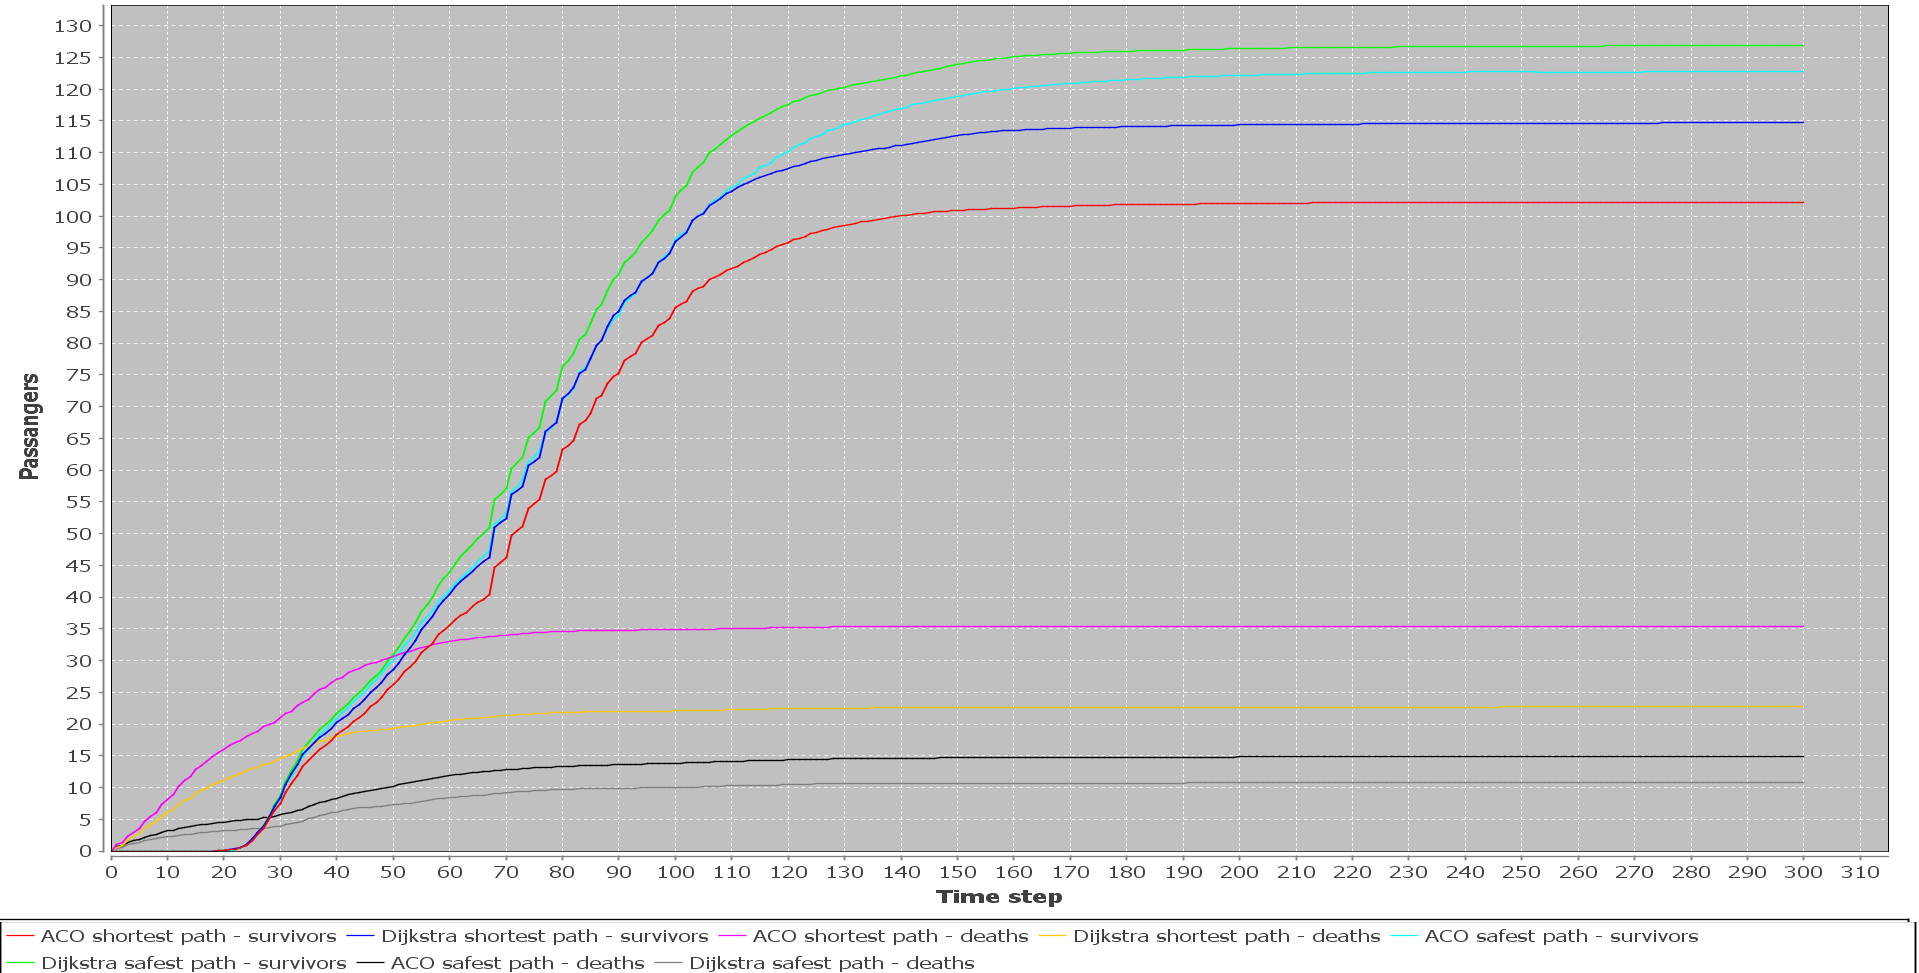
\includegraphics[scale=0.35]{images/Graph-using-1000-rounds-140-passangers.png}
\caption{Same as \ref{fig:celeb}, only using 1000 iterations.}
\label{fig:celeb1000}
\end{figure}

In the simulations there are several parameters that can be changed and multiple variables that can have an extreme impact on the simulation. For instance the fires can cover all exits and end up killing most if not all passengers. Thus each simulation runs 200 times and we obtain the average results. We found that there was no significant difference between 200 iterations and 1000 iterations as seen if one compare figure \ref{fig:celeb} with figure \ref{fig:celeb1000}.

\begin{figure} [h]
\centering
\hspace*{-1.0in}
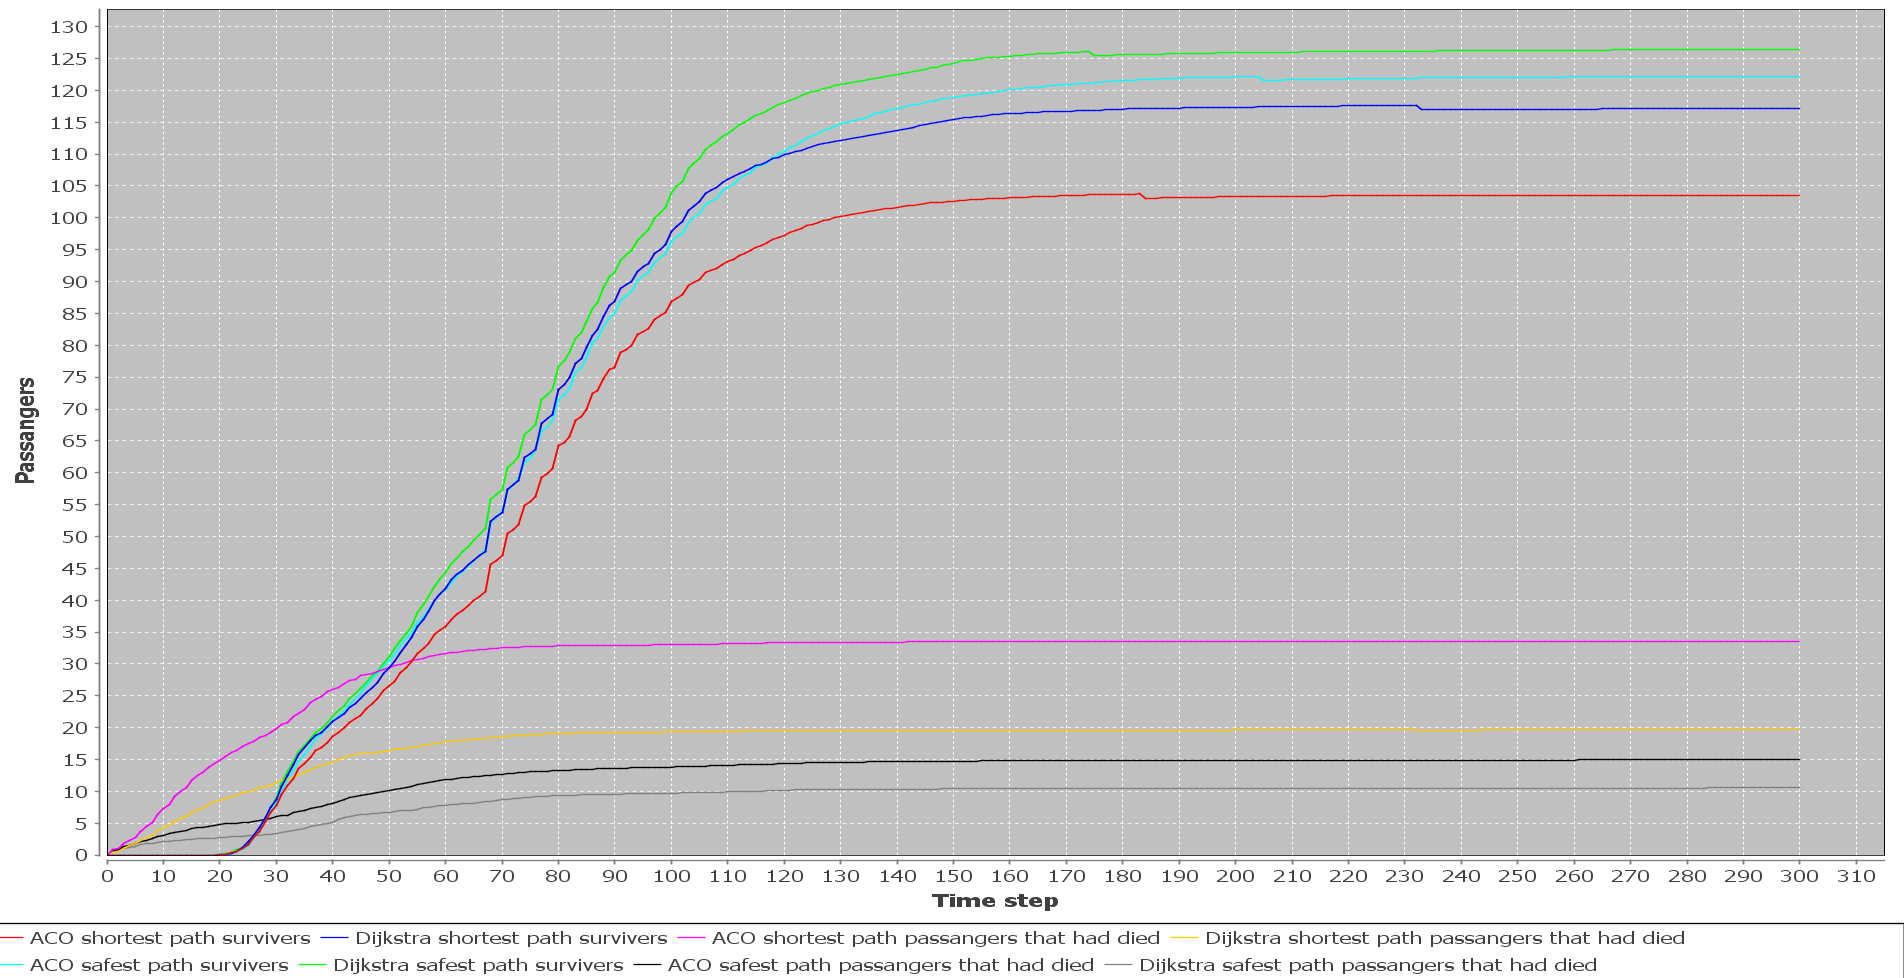
\includegraphics[scale=0.35]{images/Graph-using-200-rounds-140-passangers-and-one-fire.png}
\caption{Dijkstra and ACO running at each time step.}
\label{fig:celeb}
\end{figure}
% Crew members not accounted for
The simulations also ran with a set of standard configurations. When the effects of changing one parameter was tested the remaining ones were kept at a standard level. The number of passengers was set to the ship maximum number of passengers found on Cruisedeckplans LLC website\cite{cruseships}. The fire on board the ship was set to increase in size and intensity at every second time step, one time step being 2 real life seconds. At the start of the simulations between one and three fires were started.

At each time step ACO released 200 ants per passenger. Each ant held 200 pheromones that it used to mark the paths to the exits. The passengers would use these new paths. Similarly Dijkstra's algorithm recalculated a new path for each passenger at each timestep. In some of our simulation a few passenger would not reach the exits within 300 time steps. However we have cut the graph at 300 time steps, as this would show more details in the graph and the average number of survivors past 300 did not change. 

\section{Testing}

\subsection{Dijkstra's algorithm}

In figure \ref{fig:celebDF} we see the results of running Dijkstra's algorithm once per passenger at the start of the simulation and no more as the simulation progressed. When searching for the safest path we expected that ACO would outperform Dijkstra's algorithm, and it did. When Dijkstra's algorithm could not account for the fire spreading its performance suffered. When looking for the shortest path, ACO started out well but Dijkstra's algorithm pulled ahead after about 100 time steps. When several people occupy the same area their speed is slowed. ACO will attempt to route passengers around these areas and since Dijsktra's algorithm was only ran at the start it made no such attempts. As it turns out routing people around high occupant density areas would in general lead to a slower evacuation as a whole.

\begin{figure} [h]
\centering
\hspace*{-1.0in}
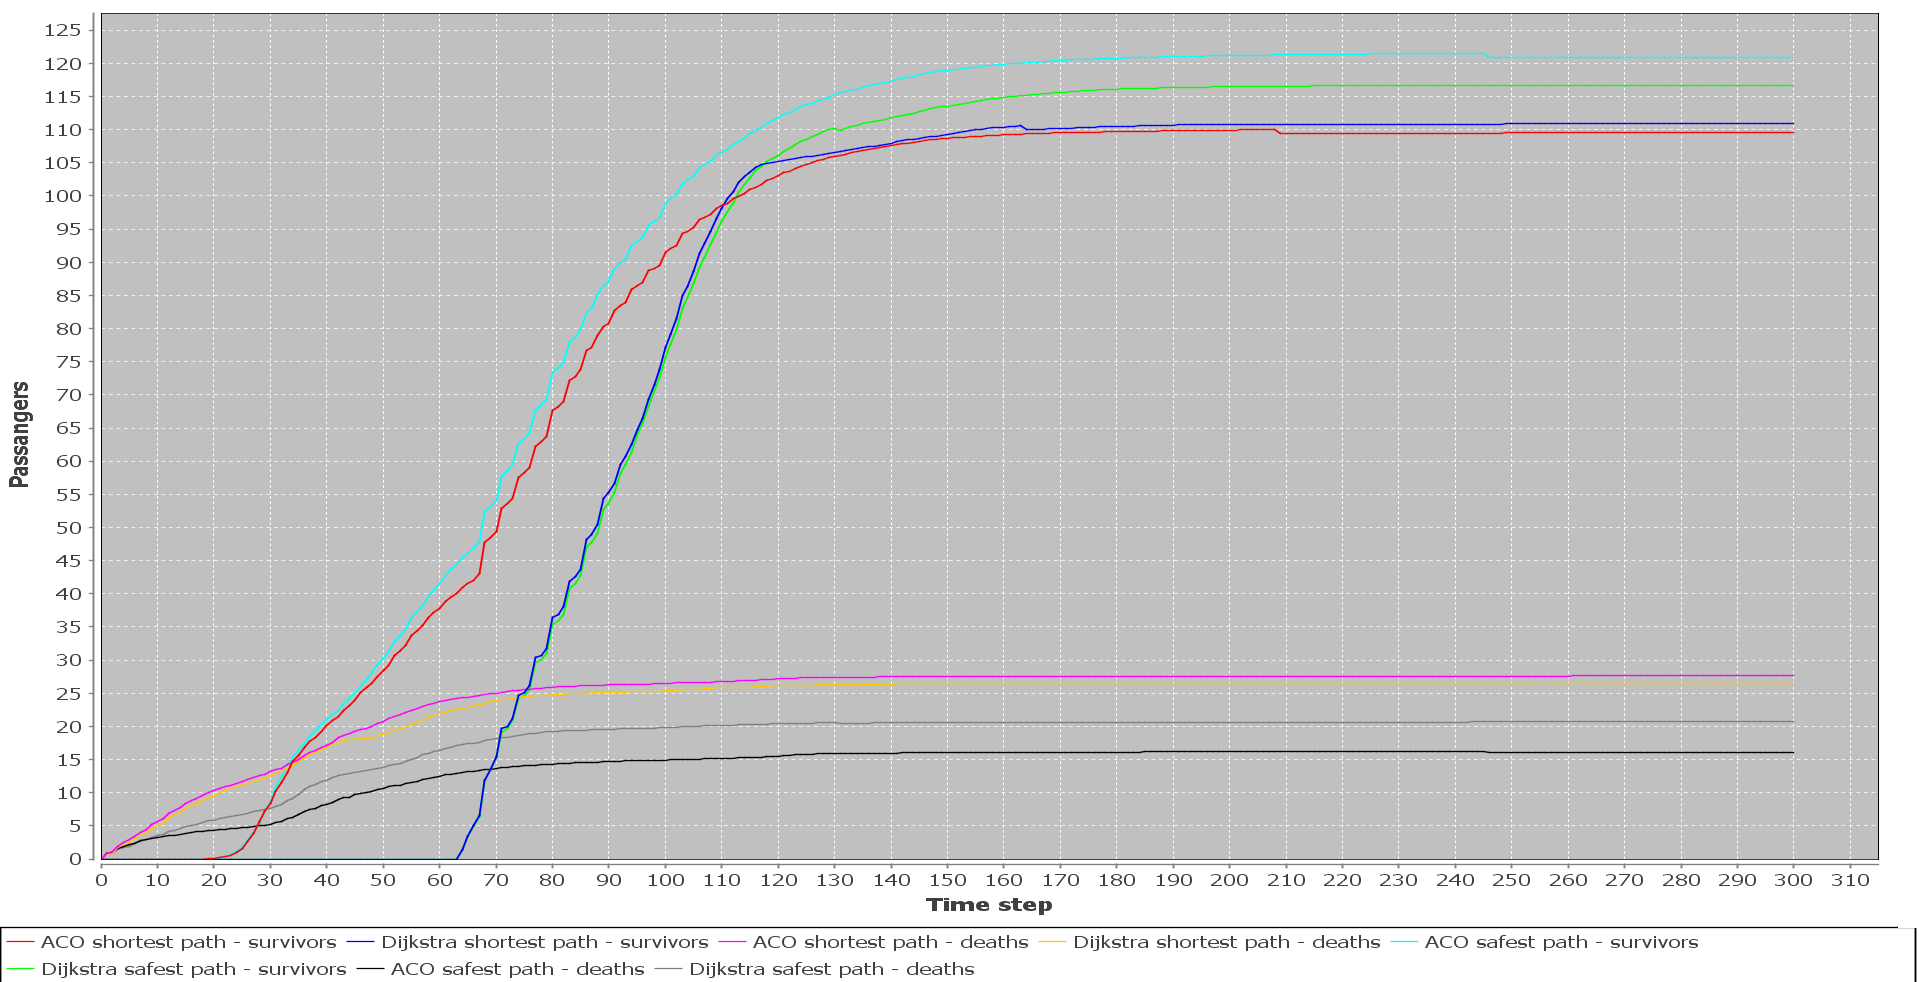
\includegraphics[scale=0.35]{images/Graph-using-1000-rounds-140-passangers-and-one-fire-dijkstra-one-time.png}
\caption{Running Dijkstra's algorithm only at start.}
\label{fig:celebDF}
\end{figure}

In figure \ref{fig:celeb} Dijkstra's algorithm was run with the standard configurations. It is clearly seen that Dijkstra's algorithm selecting the safest path has the best results overall. ACO selecting its perceived safest path would be the second best algorithm followed by Dijkstra's algorithm chosing the quickest path. ACO configured for quickest path has the worst performance, as it has problem finding the quickest path and getting the passengers off the ship before the fire spread and intensity becomes overwhelming.

% Perhaps Dijsktra's spreads less, not more?
If you look at quickest paths only, it is clearly shown that ACO's passengers are dying more rapidly then Dijkstra's passengers. This means that both algorithms are choosing different paths. As the shortest path is measured in shortest time needed to reach the exit rather than the shortest distance to exit, it would seem that Dijkstra's algorithm is more effective at spreading the passengers than ACO. Additionally Dijkstra's algorithm is able to guide passengers to an exit faster than ACO.

What is clear is that selecting the safest path is the best option regardless of algorithm. This can be atributed to the speed of the passengers and speed of the fire. If the fire spread was faster and passengers moved slower then the long and safe path around the fires could lead to the fire spreading to cover the previously safe path. Which in turn could cause more lives to be lost compared to if they took the shorter and slightly more dangerous path at the start.

%you can see how well the different algorithms did. In both cases we only used one hazard(Fire) that spread on board the ship. As shown in the graph, Dijkstra outperforms ACO in both early and late stages of this graph. In the beginning there are more passengers dying to ACO chosen path then there is in Dijkstra's chosen path, a good sign that both are finding different paths. As shortest path is measured in shortest time needed rather then shortest way to exit, it may be that Dijkstra spread the passengers more out then ACO.

%Even when more passengers are dying at the beginning of the simulations, they both have the same boost in saved passengers at each time step. The biggest problem for ACO over Dijkstra is avoiding the hazards. Shown in the graph you can see that the death toll for ACO increases faster then Dijkstra's death toll.

%In \ref{fig:celeb}, we are using the same parameters as the first one, only difference is that we are looking after the safest path rather then the shortest path for the passengers. It is clearly shown that the death toll on the passengers is far lower then the previous one. However Dijkstra proves yet again to outperform ACO in this instance. After about 30 time steps Dijkstra starts to pull ahead of ACO in number of passengers it have guided to the lifeboats. Even in number of deaths it is shown that Dijkstra is better at avoiding them. If you look at Dijkstra in both cases, the number of deaths when looking after the safest path is 50\% less when looking for the shortest path. As mention earlier that the number of rounds above 200 did not matter may be shown in the two graphs below, both of them have the same set of parameters, only to have 1000 iteration instead of 200.

%In \ref{fig:celebShortPherInEdges} and \ref{fig:celebSafePherInEdges} we tested what would the difference be if we used pheromones in edges rather then in the node themselves, this showed that the ACO preformed better then our other simulations. It was compared to Dijkstra to control that there was not something special happening. The main difference is when looking for the shortest path rather then the safest. When looking for the safest there are only some small difference in both simulations.

\begin{figure} [h]
\centering
\hspace*{-1.0in}
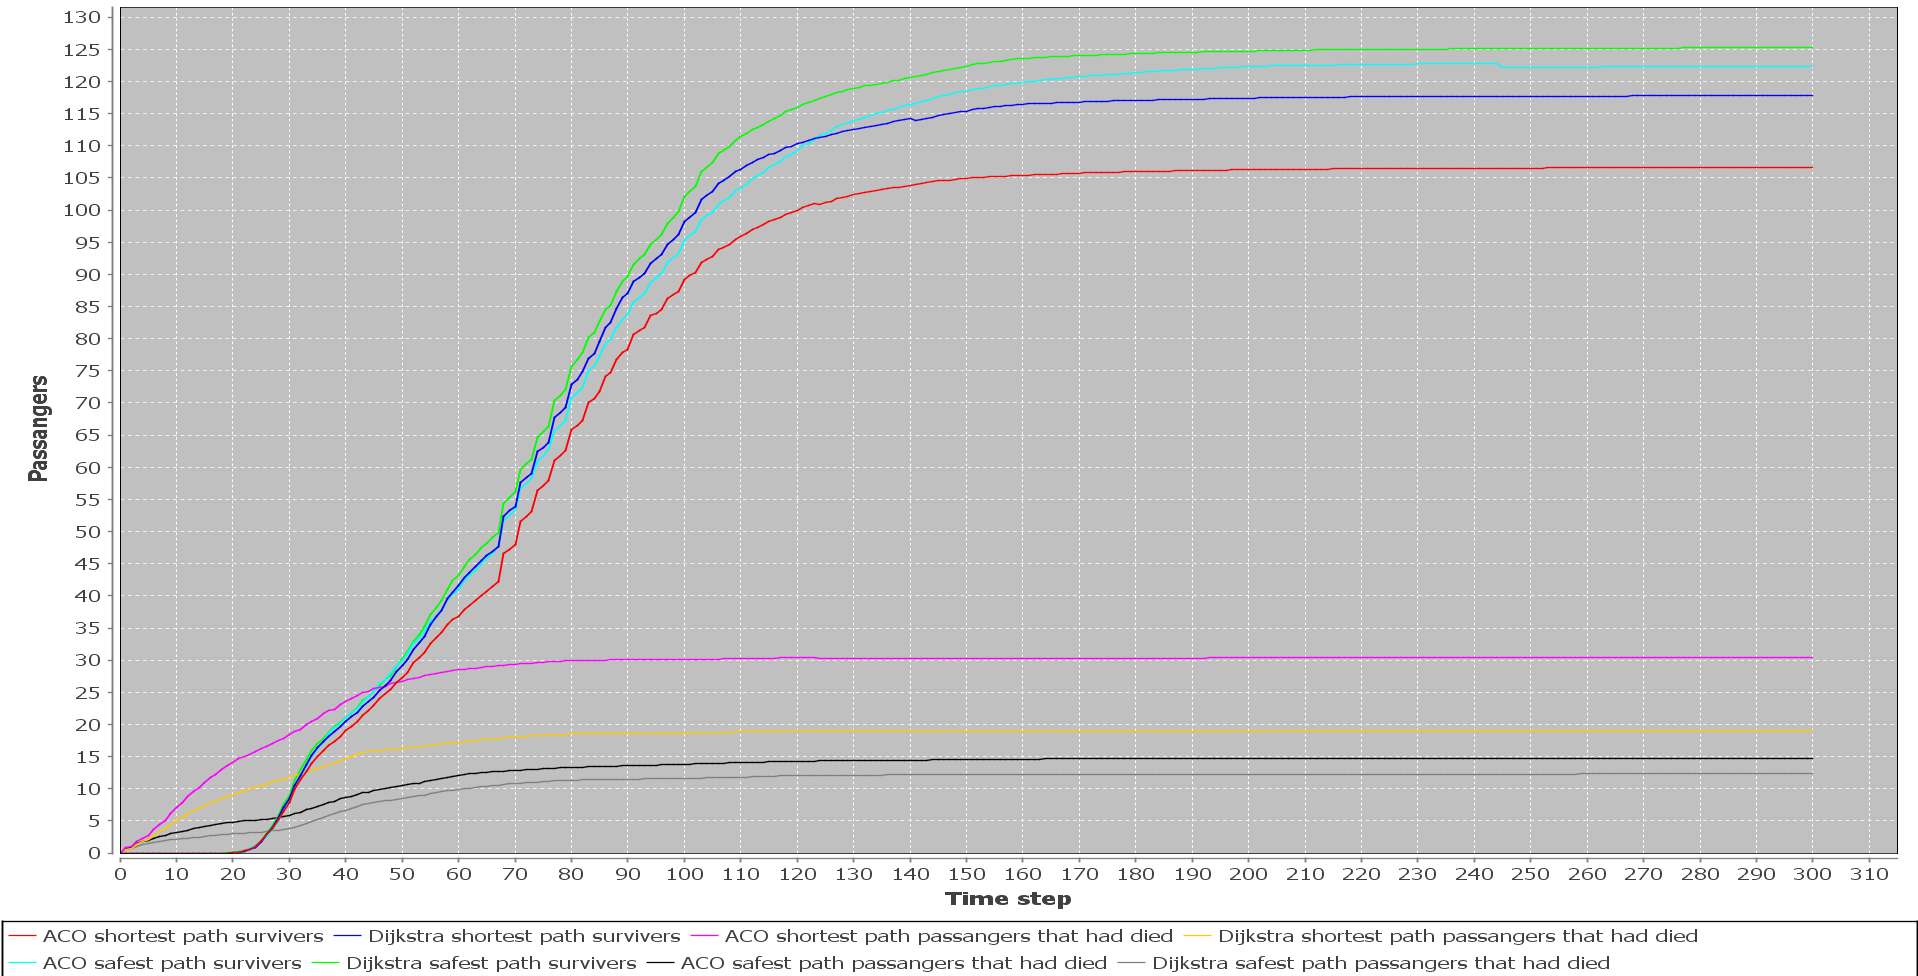
\includegraphics[scale=0.35]{images/Graph-using-200-rounds-140-passangers-and-one-hazzard-and-ACO-having-pheremons-in-edges.png}
\caption{Taking shortest path with pheromones in edges.}
\label{fig:celebPherInEdge}
\end{figure}
\subsection{Pheromones in edges}
% Ok, so do we always use pheromones in edges since it seems to be equal or better in all cases?

In \ref{fig:celebPherInEdge} we tested what would the difference be if we used pheromones in edges rather then in the node themselves, this showed that the ACO preformed just as good when going for the safest path, however when ACO was trying to go for the quickest path this had an positive effect on it and preformed better.

\begin{figure} [h]
\centering
\hspace*{-1.0in}
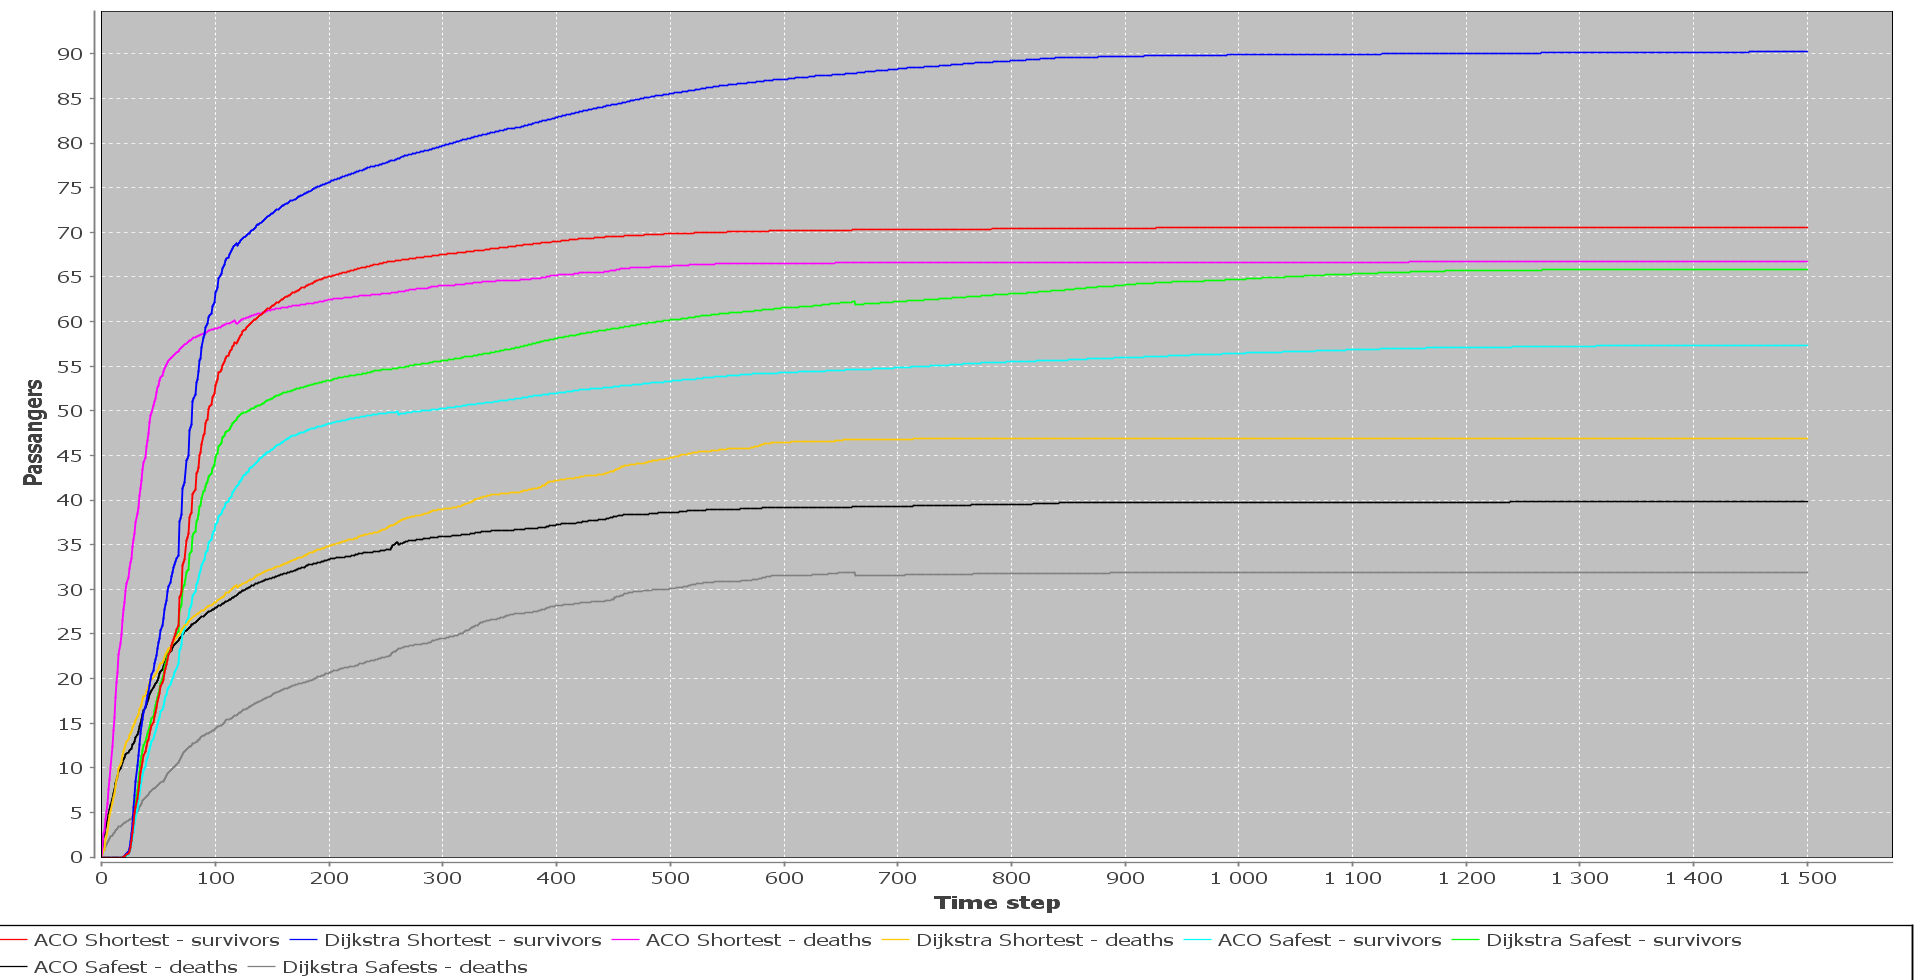
\includegraphics[scale=0.35]{images/Graph-using-200-rounds-140-passangers-and-one-fire-high-panic.png}
\caption{Taking shortest path with pheromones in edges.}
\label{fig:celebHPanic}
\end{figure}

\subsection{Higher chance of panic}
% Very interesting, get this in the conclusion
% Why would ACO not cause the same level of panic?

When the chance of panic changed to a higher chance both algorithms struggled more to guide the passengers to safety. Dijkstra had the largest drop in performance as it sometimes it would send passengers in one direction, then panic and go back, therefore taking a long time before that passenger got to safety or died. It is not clearly shown in this graph, however when it simulation was running, it resulted in a data file almost on a size of one 1 GB, where ACO's data file would not pass 60 MB. However it was also Dijkstra that preformed best overall, shown in \ref{fig:celebHPanic}.

\begin{figure} [h]
\centering
\hspace*{-1.0in}
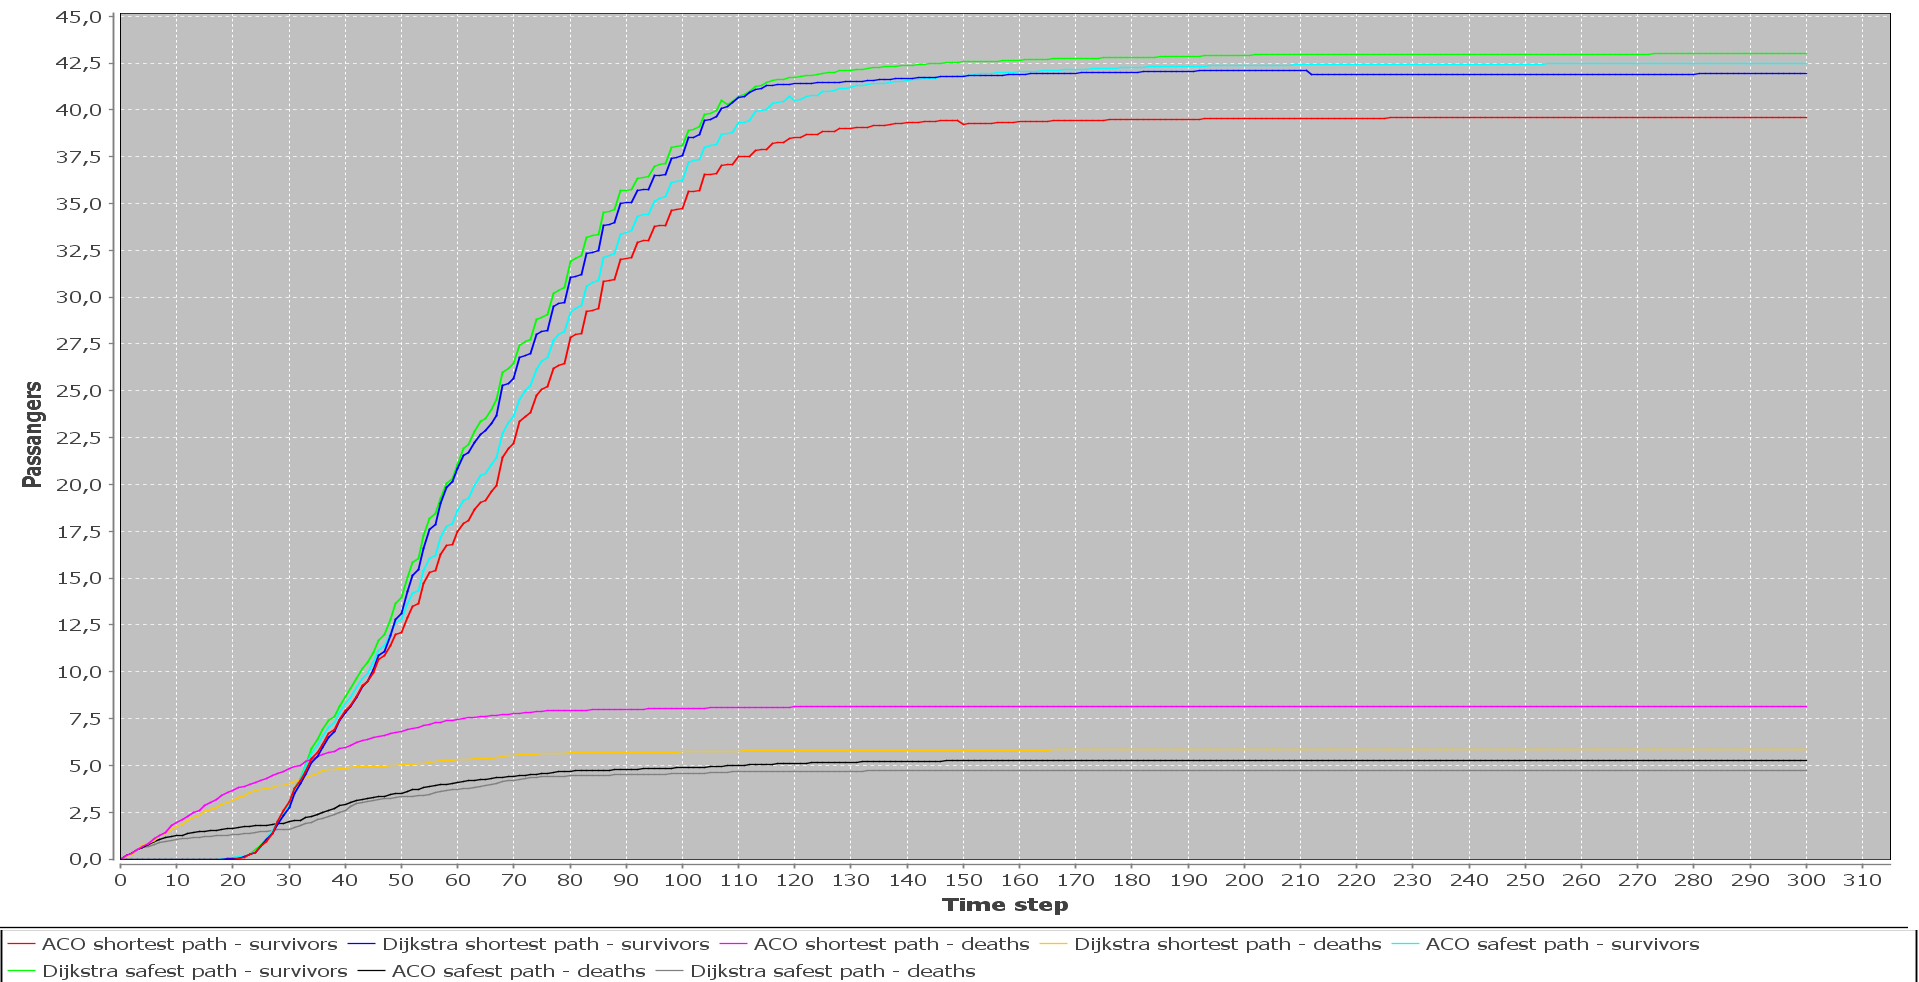
\includegraphics[scale=0.35]{images/Graph-using-200-rounds-50-passangers.png}
\caption{Taking shortest path with pheromones in edges.}
\label{fig:celeb50}
\end{figure}

\subsection{Amount of passengers}
% Do we have a section on too many passengers that we can compare to?

In \ref{fig:celeb50} all the different algorithms are close together and preform well when there are less passengers on board the ship. The order of witch algorithm that is best still remains the same, however Dijkstra going for quickest paths is just as good as ACO going for safest for a while, before ACO goes past it. When looking at the deaths of the passengers ACO going for safest is always much better then Dijkstra going for Quickest.

Again ACO's going for the quickest path is that it is a bit to slow and therefore the hazards have time to spread more out and create more dangerously areas.

\begin{figure} [h]
\centering
\hspace*{-1.0in}
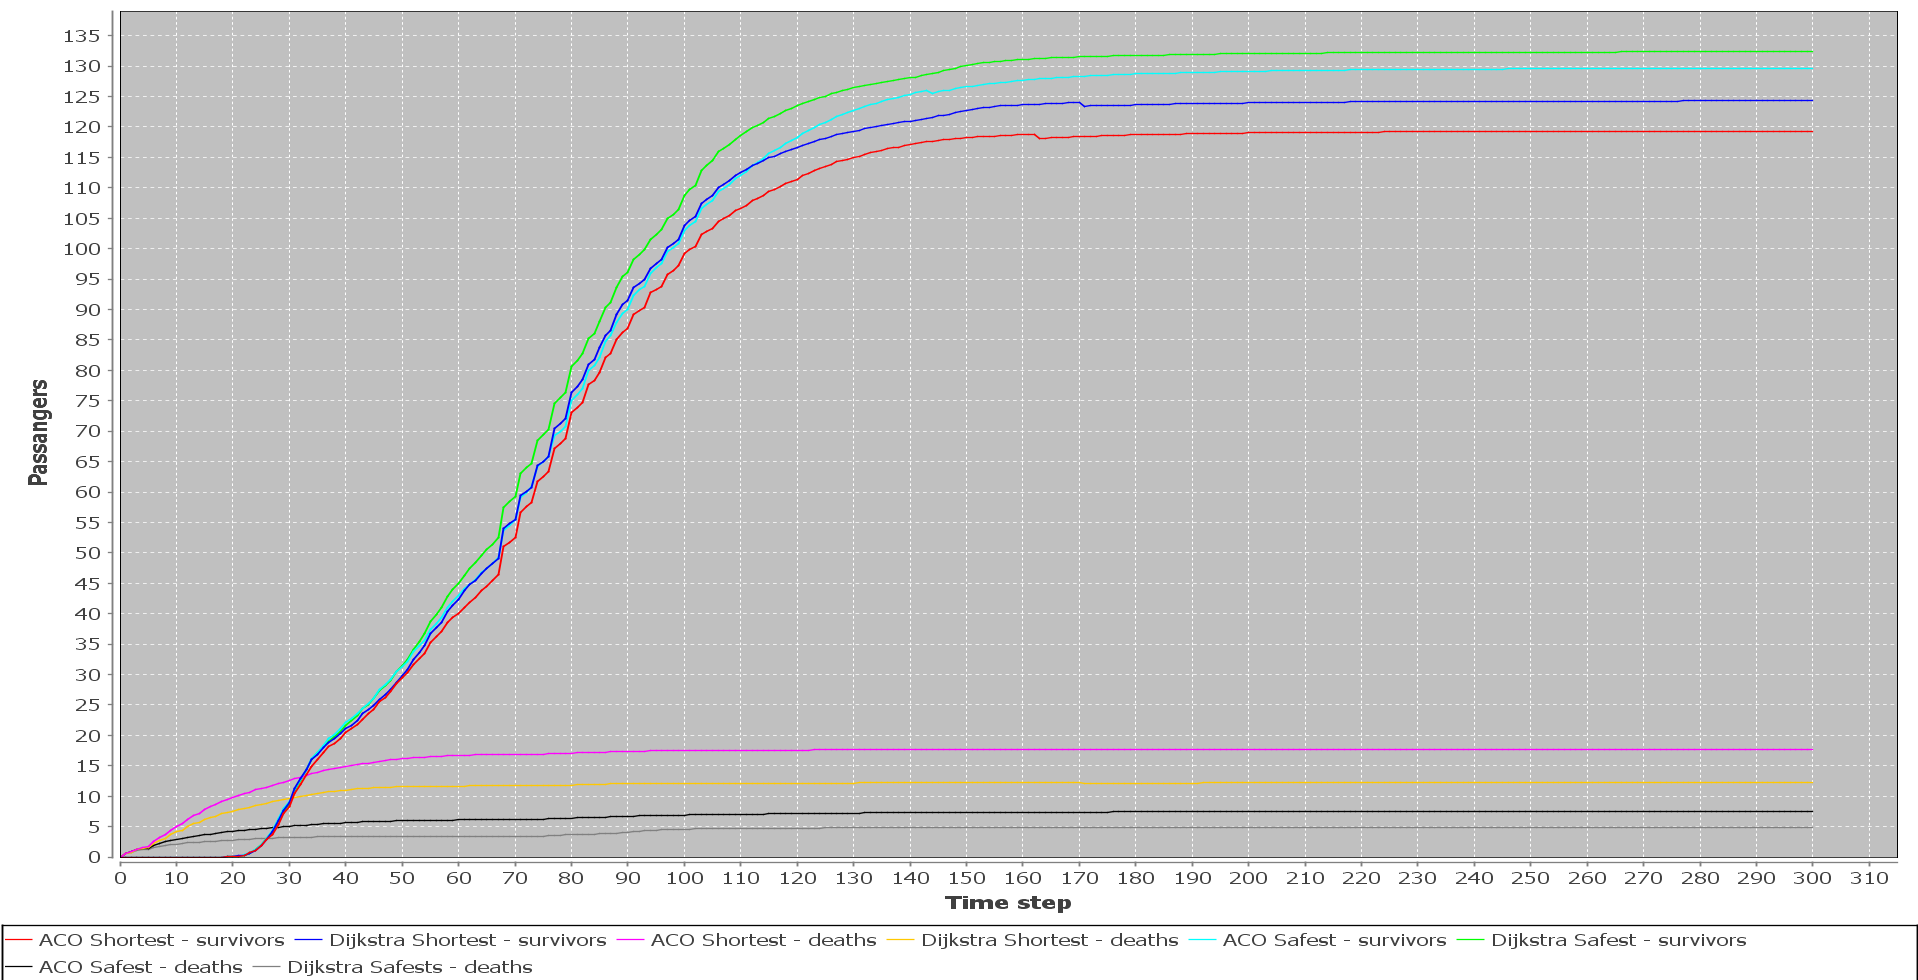
\includegraphics[scale=0.35]{images/Graph-using-200-rounds-140-passangers-slow-fire.png}
\caption{Taking shortest path with pheromones in edges.}
\label{fig:celebSfire}
\end{figure}

\subsection{Fire spread}
% Write how much slower. Reasonable that quickest path is better when there is less fire to accidentaly run into

When comparing \ref{fig:celebSfire} to \ref{fig:celeb}, the algorithms overall did much better then all the other simulations. This was expected as the hazards moved more slowly then in all the other simulations. It is also worh noting that when finding the quickest path ACO had the biggest increase in performance, however it is still the one that is the worst off.

